\documentclass{beamer}
\usetheme{Madrid} % Clean theme
\usepackage{listings}
\usepackage{xcolor}
\usepackage{graphicx}

\usepackage{gvv}

% Code listing style
\lstset{
  basicstyle=\ttfamily\footnotesize,
  keywordstyle=\color{blue},
  stringstyle=\color{orange},
  commentstyle=\color{green!60!black},
  breaklines=true,
  frame=single,
  showstringspaces=false
}

\title{MatGeo Assignment - Problem 4.3.9}
\author{EE25BTECH11024}
\institute{IIT Hyderabad}

\begin{document}

% Title slide
\begin{frame}
  \titlepage
\end{frame}

% Problem statement
\begin{frame}{Problem Statement}
The vector equation of the line
\begin{align}
\frac{x - 5}{3} = \frac{y + 4}{7} = \frac{z - 6}{2}
\label{eq:given}
\end{align}
is \_\_\_\_\_\_\_\_\_\_\_\_\_.
\end{frame}


\begin{frame}{Formula Used}
    The general vector equation of a line in 3D is
\begin{align}
\vec{x} = \vec{h} + \kappa \vec{m},   
\label{eq:formula}
\end{align}
    
\end{frame}

\begin{frame}{Solution: }
\noindent
From \eqref{eq:given} we get the following equations.
\begin{align}
    x &= 5 + 3\kappa, \label{eq:a} \\ 
    y &= -4 + 7\kappa, \label{eq:b} \\ 
    z &= 6 + 2\kappa. \label{eq:c}
\end{align}
comparing \eqref{eq:a}, \eqref{eq:b}, \eqref{eq:c}, and \eqref{eq:formula} we get,
\begin{align}
\vec{h} = \myvec{5 \\ -4 \\ 6}, \quad 
\vec{m} = \myvec{3 \\ 7 \\ 2}.    
\end{align}
\end{frame}


\begin{frame}{Final Answer}
\noindent
\textbf{Therefore, the vector equation of the line is:}
\begin{align}
\vec{x} = \myvec{5 \\ -4 \\ 6} + \kappa \myvec{3 \\ 7 \\ 2}
\end{align}

See Figure~\ref{fig:3DVectors}.   
\end{frame}

\begin{frame}{Figure}
    \begin{figure}[h!]
    \centering
    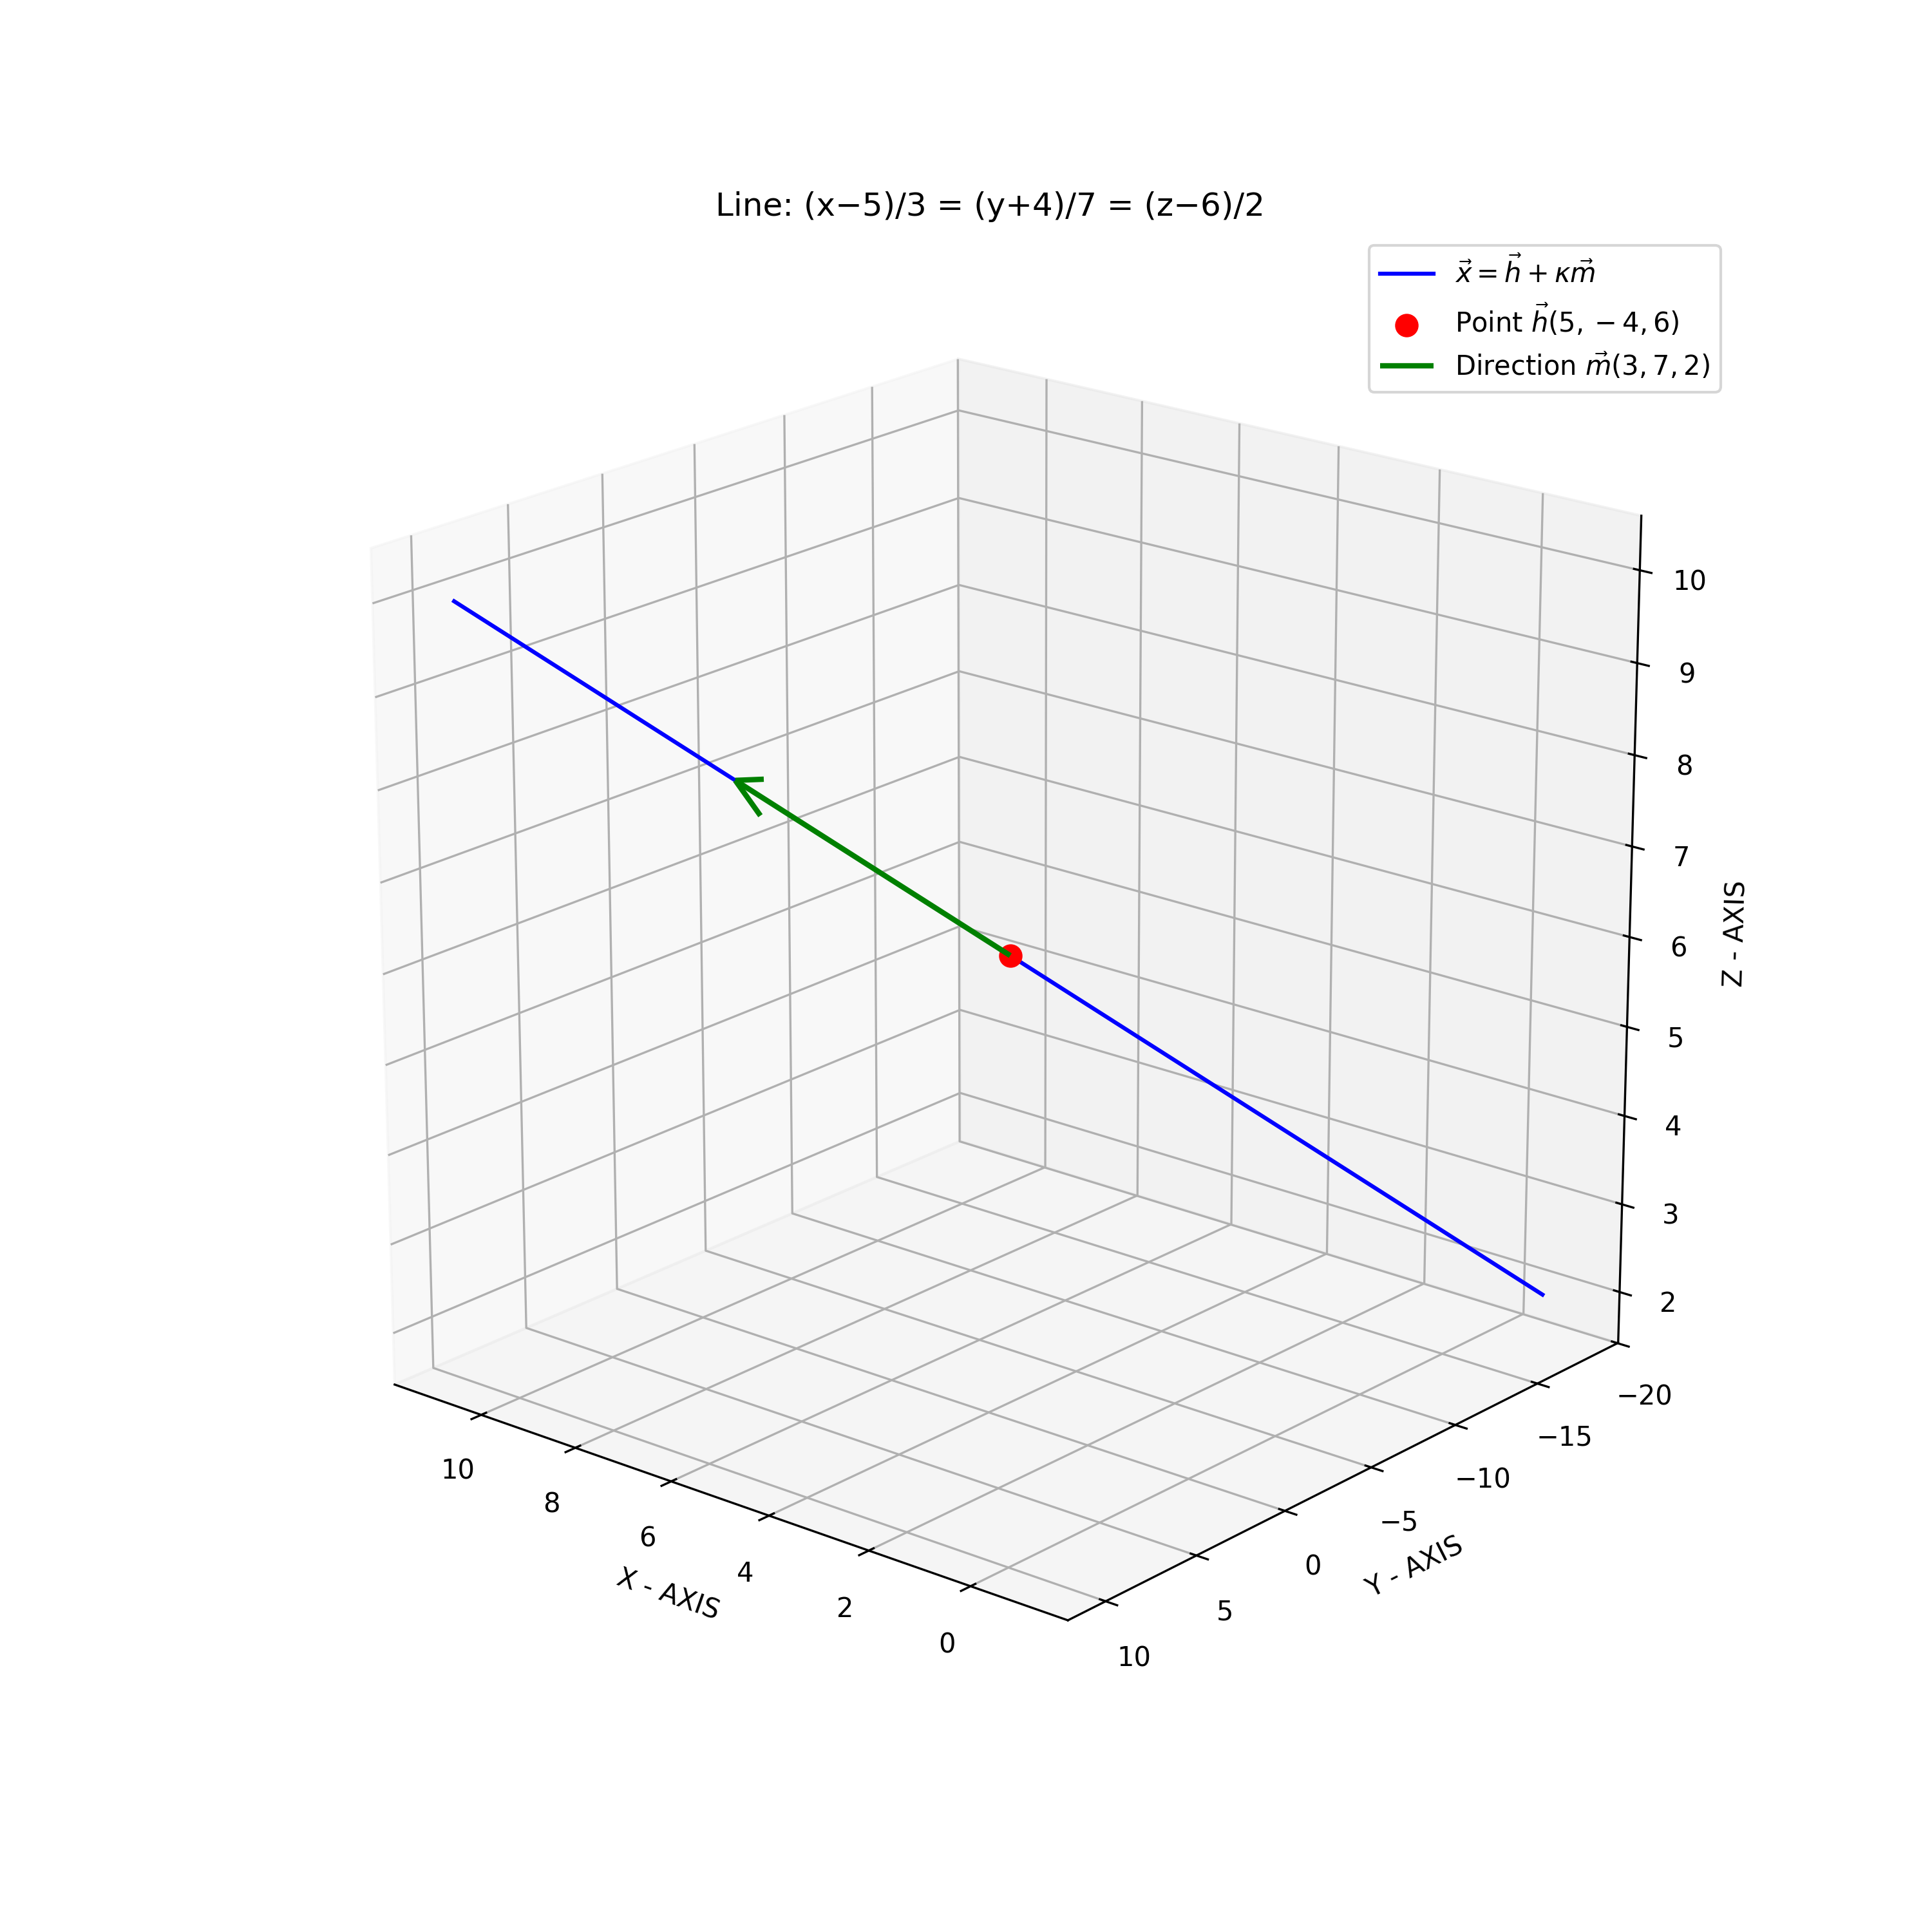
\includegraphics[width=0.7\linewidth]{figs/fig.png}
    \caption{}
    \label{fig:3DVectors}
\end{figure}
\end{frame}

% Python code 1
\begin{frame}[fragile]{Python Code: plot.py (Native)}
\begin{lstlisting}[language=Python]
import numpy as np
import matplotlib.pyplot as plt
from mpl_toolkits.mplot3d import Axes3D

h = np.array([5, -4, 6])  
m = np.array([3, 7, 2])  

k_values = np.linspace(-2, 2, 100)
line_points = np.array([h + k * m for k in k_values])

fig = plt.figure(figsize=(10,10))
ax = fig.add_subplot(111, projection='3d')

ax.plot(line_points[:,0], line_points[:,1], line_points[:,2], color='blue', label=r"$\vec{x} = \vec{h} + \kappa \vec{m}$")

ax.scatter(h[0], h[1], h[2], color='red', s=60, label=r"Point $\vec{h}(5, -4, 6)$")
\end{lstlisting}
\end{frame}


\begin{frame}[fragile]{Python Code (Native Implementation – plot.py)}
\begin{lstlisting}[language=Python]
ax.quiver(h[0], h[1], h[2], m[0], m[1], m[2], 
          color='green', arrow_length_ratio=0.1, linewidth=2, label=r"Direction $\vec{m}(3,7,2)$")

ax.set_xlabel("X - AXIS")
ax.set_ylabel("Y - AXIS")
ax.set_zlabel("Z - AXIS")
ax.set_title("Line: (x−5)/3 = (y+4)/7 = (z−6)/2")
ax.legend()
ax.set_box_aspect([1,1,1]) 
ax.view_init(elev=20, azim=130)
plt.savefig("line_vector_equation.png", dpi=300)
plt.show()
\end{lstlisting}
\end{frame}


\begin{frame}[fragile]{C Code (Shared Library – findlinepoints.c)}
\begin{lstlisting}[language=C]
#include <stdio.h>

void find_line_points(double *h, double *m, double k1, double k2, double *P1, double *P2)
{
    for (int i = 0; i < 3; i++) {
        P1[i] = h[i] + k1 * m[i];
        P2[i] = h[i] + k2 * m[i];
    }
}

\end{lstlisting}
\end{frame}

% Python code 2
\begin{frame}[fragile]{Python Code: call.py (C + Python)}
\begin{lstlisting}[language=Python]
import ctypes
import numpy as np
import matplotlib.pyplot as plt
from mpl_toolkits.mplot3d import Axes3D

lib = ctypes.CDLL("./find_line_points.so")

lib.find_line_points.argtypes = [
    ctypes.POINTER(ctypes.c_double),  
    ctypes.POINTER(ctypes.c_double),  
    ctypes.c_double,                  
    ctypes.c_double,                  
    ctypes.POINTER(ctypes.c_double),  
    ctypes.POINTER(ctypes.c_double)   
]
lib.find_line_points.restype = None

h = np.array([5.0, -4.0, 6.0], dtype=np.float64)
m = np.array([3.0, 7.0, 2.0], dtype=np.float64)
\end{lstlisting}
\end{frame}

\begin{frame}[fragile]{Python Code (C Integrated – call.py)
}
\begin{lstlisting}[language=Python]
P1 = np.zeros(3, dtype=np.float64)
P2 = np.zeros(3, dtype=np.float64)

k1, k2 = -2.0, 2.0
lib.find_line_points(h.ctypes.data_as(ctypes.POINTER(ctypes.c_double)),
                     m.ctypes.data_as(ctypes.POINTER(ctypes.c_double)),
                     k1, k2,
                     P1.ctypes.data_as(ctypes.POINTER(ctypes.c_double)),
                     P2.ctypes.data_as(ctypes.POINTER(ctypes.c_double)))

line_points = np.linspace(P1, P2, 100)

fig = plt.figure(figsize=(10,10))
ax = fig.add_subplot(111, projection='3d')

ax.plot(line_points[:,0], line_points[:,1], line_points[:,2], color='blue', label=r"$\vec{x} = \vec{h} + \kappa \vec{m}$")

ax.scatter(h[0], h[1], h[2], color='red', s=60, label=r"Point $\vec{h}(5, -4, 6)$")
\end{lstlisting}
\end{frame}

\begin{frame}[fragile]{Python Code (C Integrated – call.py)
}
\begin{lstlisting}[language=Python]
ax.quiver(h[0], h[1], h[2], m[0], m[1], m[2],
          color='green', arrow_length_ratio=0.1, linewidth=2, label=r"Direction $\vec{m}(3,7,2)$")

ax.set_xlabel("X - AXIS")
ax.set_ylabel("Y - AXIS")
ax.set_zlabel("Z - AXIS")
ax.set_title("Line: (x−5)/3 = (y+4)/7 = (z−6)/2")
ax.legend()
ax.set_box_aspect([1,1,1])  # Equal aspect ratio
ax.view_init(elev=20, azim=130)
plt.savefig("line_vector_equation_from_dll.png", dpi=300)
plt.show()
\end{lstlisting}
\end{frame}


\end{document}


